\documentclass[11pt]{article}
% Template for PLoS
% Version 3.2 March 2016

% General commands for the entire paper
%
% Use Unicode characters when possible
\usepackage[utf8x]{inputenc}
% amsmath package, useful for mathematical formulas
\usepackage{amsmath}
%\usepackage{natbib}
% amssymb package, useful for mathematical symbols
\usepackage{amssymb}
\usepackage{booktabs}
\usepackage{xspace}
\usepackage{hyperref}
% graphicx package, useful for including eps and pdf graphics
% include graphics with the command \includegraphics
\usepackage{graphicx}

% Use adjustwidth environment to exceed column width (see example table in text)
\usepackage{changepage}

% textcomp package and marvosym package for additional characters
\usepackage{textcomp,marvosym}

% fixltx2e package for \textsubscript
\usepackage{fixltx2e}

% cite package, to clean up citations in the main text. Do not remove.
\usepackage{cite}
\usepackage{caption}
\usepackage{subcaption}
\usepackage{rotating}

\usepackage{color}

% Use doublespacing - comment out for single spacing
%\usepackage{setspace}
%\doublespacing

% Text layout
\topmargin 0.0cm
\oddsidemargin 0.5cm
\evensidemargin 0.5cm
\textwidth 16cm
\textheight 21cm

\setlength{\parskip}{1em}

% Bold the 'Figure #' in the caption and separate it with a period
% Captions will be left justified
\usepackage[labelfont=bf,labelsep=period,justification=raggedright]{caption}

% Use the PLoS provided bibtex style
\bibliographystyle{/Users/stephens/Dropbox/Documents/stylefiles/plos2009}

% Remove brackets from numbering in List of References
\makeatletter
\renewcommand{\@biblabel}[1]{\quad#1.}
\makeatother

% Use nameref to cite supporting information files (see Supporting Information section for more info)
\usepackage{nameref,hyperref}

% line numbers
\usepackage[right]{lineno}

% ligatures disabled
\usepackage{microtype}
\DisableLigatures[f]{encoding = *, family = * }

% Leave date blank
\date{}

\pagestyle{myheadings}
%% ** EDIT HERE **
\usepackage{enumerate}
\usepackage{multirow}
\usepackage{url}
\usepackage{xr} %for cross-referencing
%% ** EDIT HERE **
%% PLEASE INCLUDE ALL MACROS BELOW
\newtheorem{algorithm}{Algorithm}
\newtheorem{proposition}{Proposition}
\newtheorem{restateproposition}{Proposition}
\newtheorem{lemma}{Lemma}
\newtheorem{corollary}{Corollary}
\newtheorem{result}{Result}
\newtheorem{note}{Note}
\newtheorem{definition}{Definition}

\def\KL{\text{KL}}


% Text layout
\raggedright
\setlength{\parindent}{0.5cm}
\textwidth 5.25in
\textheight 8.75in

% Bold the 'Figure #' in the caption and separate it from the title/caption with a period
% Captions will be left justified
\usepackage[aboveskip=1pt,labelfont=bf,labelsep=period,justification=raggedright,singlelinecheck=off]{caption}
\renewcommand{\figurename}{Fig}

%------ bibliography
% Use the PLoS provided BiBTeX style
\bibliographystyle{plos2015}
% Remove brackets from numbering in List of References
\makeatletter
\renewcommand{\@biblabel}[1]{\quad#1.}
\makeatother


% Header and Footer with logo
\usepackage{lastpage,fancyhdr,graphicx}
\usepackage{epstopdf}
\pagestyle{myheadings}
\pagestyle{fancy}
\fancyhf{}
\setlength{\headheight}{27.023pt}
\lhead{\includegraphics[width=2.0in]{PLOS-submission.eps}}
\rfoot{\thepage/\pageref{LastPage}}
\renewcommand{\footrule}{\hrule height 2pt \vspace{2mm}}
\fancyheadoffset[L]{2.25in}
\fancyfootoffset[L]{2.25in}
\lfoot{\sf PLOS}

%% Include all macros below

\newcommand{\lorem}{{\bf LOREM}}
\newcommand{\ipsum}{{\bf IPSUM}}

%% END MACROS SECTION

%% Author's settings
\def\KL{\text{KL}}

\begin{document}

\section{Hierarchical and Admixture model comparison}

In order to compare between the hierarchical and admixture models, we first draw from the entire pool of $648$ Heart Left Ventricle and Muscle Skeletal samples, a  set of 50 samples, some of which are Heart Left Ventricle and some are Muscle Skeletal. Now ideally our method should separate out the Heart Left Ventricle and the Muscle Skeletal samples. So, if we code Heart Left Ventricle as 1 and Muscle Skeletal as 0, then ideally after arrangement in a heatmap and once we have arranged the samples as per their clustering in the heatmap, we would expect the following ordering $t_1 =(1,1,1.\cdots, 1, 0,0,0, \cdots, 0)$ or $t_2 = (0,0,0, \cdots, 0, 1,1,1, \cdots,1)$. These two vectors would imply complete separation of the two tissues. However, in general using hierarchical clustering or admixture, we will get some permutation of the above vectors where the number of $1$ s and the number of $0$ s would remain the same but the above patterns may not be maintained. Let us assume that the ordering we get by hierarchical clustering on the $50$ samples be $c_{H}$ and that under admixture be $c_{A}$. Then we would want to see how close these two vectors are to either of $t_1$. So, we define the misclassification proportion for hierarchical model and the admixture model as 

$$ m_H = min \left( ||c_{H} - t_{1} ||_{0}, ||c_{H} - t_{2} ||_{0}  \right )  $$
$$ m_A = min \left( ||c_{A} - t_{1} ||_{0}, ||c_{A} - t_{2} ||_{0}  \right )  $$

Then we run $200$ runs of drawing random samples of size $50$ as above and obtaining $m_H$ and $m_A$ and then plot $m_H$ against $m_A$. 

The following figure depicts it for 50 samples case. I think we should repeat this with more number of samples per batch- may be 200 or 300 but it seems that Admixture is doing far better than the Hierarchical model from just these runs.

\begin{figure*}[ht]
	\centering
	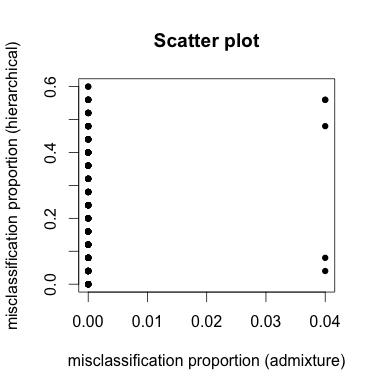
\includegraphics[height=2.5in, width=2.5in]{../plots/misclass_compare_admixture_hierarchy.png}
        \caption{Comparison of the misclassification error for the Admixture model and the Hierarchical model both under average linkage and using Euclidean distance of separation.}
\end{figure*}


\end{document}





